\documentclass[12pt]{article}

% Load packages
\usepackage{url}  % Formatting web addresses
\usepackage{ifthen}  % Conditional
\usepackage{multicol}   %Columns
\usepackage[utf8]{inputenc} %unicode support
\usepackage{amsmath}
\usepackage{amssymb}
\usepackage{epsfig}
\usepackage{epstopdf}
\usepackage{graphicx}
\usepackage{cite}
\usepackage{lastpage,fancyhdr,graphicx}
\usepackage{mathtools}
\usepackage[margin=0.1pt,font=footnotesize,labelfont=bf]{caption}
\usepackage{setspace}
%\usepackage{longtable}
\usepackage{colortbl}
%\usepackage{palatino,lettrine}
%\usepackage{times}
%\usepackage[applemac]{inputenc} %applemac support if unicode package fails
%\usepackage[latin1]{inputenc} %UNIX support if unicode package fails
\usepackage[wide]{sidecap}
%\usepackage[authoryear,round,comma,sort&compress]{natbib}
\usepackage[square,sort,comma,numbers,sort&compress]{natbib}
%\usepackage[authoryear,round]{natbib}
\usepackage{supertabular}
\usepackage{fullpage}
\usepackage{comment}
\usepackage{lineno}
%\usepackage{chicago}
\usepackage{textcomp}
\usepackage{multirow}
\usepackage{amsmath}
\usepackage{color}
\usepackage{booktabs}
\usepackage{xfrac}
\usepackage{afterpage}
\usepackage{placeins}
\setlength\heavyrulewidth{0.4ex}
\setlength\lightrulewidth{0.25ex}
%\usepackage{textgreek}
%\usepackage[linesnumbered,lined,boxed,commentsnumbered]{algorithm2e}
\DeclareMathOperator*{\argmin}{\arg\!\min}

%\usepackage{algorithm2e}
%\usepackage{algpseudocode}
%\usepackage[space]{cite}
\urlstyle{rm}
\hyphenation{dec-ades} %Latex does not know how to hyphenate this by default, so we add it to the list
\def\wl{\par \vspace{\baselineskip}}

%\textwidth = 6.50 in
%\textheight = 9.5 in
%\oddsidemargin =  0.0 in
%\evensidemargin = 0.0 in
%\topmargin = -0.50 in
%\headheight = 0.0 in
%\headsep = 0.25 in
%\parskip = 0.15in
%\linespread{1.75}
\doublespace

%\bibliographystyle{chicago}
\bibliographystyle{plos2015}

\makeatletter
\renewcommand\subsection{\@startsection
	{subsection}{2}{0mm}
	{-0.05in}
	{-0.5\baselineskip}
	{\normalfont\normalsize\bfseries}}
\renewcommand\subsubsection{\@startsection
	{subsubsection}{2}{0mm}
	{-0.05in}
	{-0.5\baselineskip}
	{\normalfont\normalsize\itshape}}
\renewcommand\section{\@startsection
	{subsection}{2}{0mm}
	{-0.2in}
	{0.05\baselineskip}
	{\normalfont\large\bfseries}}
\renewcommand\paragraph{\@startsection
	{paragraph}{2}{0mm}
	{-0.05in}
	{-0.5\baselineskip}
	{\normalfont\normalsize\itshape}}
\makeatother

% Single space'd bib -
\setlength\bibsep{0pt}

\renewcommand{\rmdefault}{phv}\renewcommand{\sfdefault}{phv}
\newcommand{\norm}[1]{\left\lVert#1\right\rVert}

% Change the number format in the ref list -
\renewcommand{\bibnumfmt}[1]{#1.}

% Change Figure to Fig.
\renewcommand{\figurename}{Fig.}

% Begin ...
\begin{document}

%\date{}
%\thispagestyle{empty}
%\pagebreak

\setcounter{page}{1}
\linenumbers

%\section*{Introduction}
%Mathematical modeling has long contributed to our understanding of metabolism.
%Decades before the genomics revolution, mechanistically structured metabolic models arose from the desire to predict microbial phenotypes resulting from changes in intracellular or extracellular states \textit{1976-fredrickson}.
%The single cell \textit{E. coli} models of Shuler and coworkers pioneered the construction of large-scale, dynamic metabolic models that incorporated multiple regulated catabolic and anabolic pathways constrained by experimentally determined kinetic parameters \textit{1984-domach-shuler-BiotechBioeng-01}.
%Shuler and coworkers generated many single cell kinetic models, including single cell models of eukaryotes \textit{1989-steinmeyer,1992-wu}, minimal cell architectures \textit{2004-castellanos}, as well as DNA sequence based whole-cell models of \textit{E. coli} \textit{2008-atlas-shuler-IETSysBio}.
%\clearpage

\section*{Overview}

%\clearpage

\section*{Balance equations}

%\subsection*{Formulation and solution of the model equations.} 
%We used ordinary differential equations (ODEs) to model the time evolution of metabolite ($x_{i}$) and scaled enzyme abundance ($\epsilon_{i}$) in hypothetical cell-free metabolic networks:
%\begin{eqnarray}
%	\frac{dx_{i}}{dt} & = & \sum_{j=1}^{\mathcal{R}}\sigma_{ij}r_{j}\left(\mathbf{x},\mathbf{\epsilon},\mathbf{k}\right)\qquad{i=1,2,\hdots,\mathcal{M}}\\
%	\frac{d\epsilon_{i}}{dt} & = & -\lambda_{i}\epsilon_{i}\qquad{i=1,2,\hdots,\mathcal{E}}
%\end{eqnarray}where $\mathcal{R}$ denotes the number of reactions, $\mathcal{M}$ denotes the number of metabolites and $\mathcal{E}$ denotes the number of enzymes in the model.
%The quantity $r_{j}\left(\mathbf{x},\mathbf{\epsilon},\mathbf{k}\right)$ denotes the rate of reaction $j$.
%Typically, reaction $j$ is a non-linear function of metabolite and enzyme abundance, as well as unknown kinetic parameters $\mathbf{k}$ ($\mathcal{K}\times{1}$).
%The quantity $\sigma_{ij}$ denotes the stoichiometric coefficient for species $i$ in reaction $j$.
%If $\sigma_{ij}>0$, metabolite $i$ is produced by reaction $j$.
%Conversely, if $\sigma_{ij}<0$, metabolite $i$ is consumed by reaction $j$, while $\sigma_{ij}=0$ indicates metabolite $i$ is not connected with reaction $j$.
%Lastly, $\lambda_{i}$ denotes the scaled enzyme activity decay constant.
%The system material balances were subject to the initial conditions $\mathbf{x}\left(t_{o}\right)=\mathbf{x}_{o}$ and $\mathbf{\epsilon}\left(t_{o}\right)=\mathbf{1}$ (initially we have 100\% cell-free enzyme abundance).

%The reaction rate was written as the product of a kinetic term ($\bar{r}_{j}$) and a control term ($v_{j}$), $r_{j}\left(\mathbf{x},\mathbf{k}\right)=\bar{r}_{j}v_{j}$.
%We used multiple saturation kinetics to model the reaction term $\bar{r}_{j}$:
%\begin{equation}\label{eqn:rate-bar}
%	\bar{r}_{j}=V_{j}^{max}\epsilon_{i}\prod_{s\in{m_{j}^{-}}}\frac{x_{s}}{K_{js} + x_{s}}
%\end{equation}
%where $V_{j}^{max}$ denotes the maximum rate for reaction $j$, $\epsilon_{i}$ denotes the scaled enzyme activity which catalyzes reaction $j$, $K_{js}$ denotes the saturation constant for species $s$, in reaction $j$ and $m_{j}^{-}$ denotes the set of \textit{reactants} for reaction $j$.
%Transcription was modeled as first-order in RNA polymerase, since it acts like an enzyme:
%\begin{equation}\label{eqn:transcription}
%    \bar{r}^{TX} = k_{cat}^{TX}\cdot{\rm RNAP}\left(\frac{{\rm GENE}}{K_{GENE}^{TX}+{\rm GENE}}\right)\prod_{s\in{m_{TX}^{-}}}\frac{x_{s}}{K_{s}^{TX}+x_{s}}
%\end{equation}
%where $k_{cat}^{TX}$ denotes the maximum transcription rate, ${\rm RNAP}$ denotes the RNA polymerase concentration, $GENE$ denotes the gene concentration, $K_{GENE}^{TX}$ denotes the gene saturation constant, $K_{s}^{TX}$ denotes the saturation constant for species $s$, and $m_{TX}^{-}$ denotes the set of \textit{reactants} for transcription: ATP, GTP, CTP, UTP, and water.
%While transcription is modeled as saturating with respect to gene concentration, the gene is not considered a reactant in the stoichiometry as it is not consumed.
%Translation was modeled as first-order in ribosome, since it acts like an enzyme:
%\begin{equation}\label{eqn:translation}
%    \bar{r}^{TL} = k_{cat}^{TL}\cdot{\rm RIBO}\left(\frac{{\rm mRNA}}{K_{mRNA}^{TL}+{\rm mRNA}}\right)\prod_{s\in{m_{TL}^{-}}}\frac{x_{s}}{K_{s}^{TL}+x_{s}}
%\end{equation}
%where $k_{cat}^{TL}$ denotes the maximum translation rate, ${\rm RIBO}$ denotes the ribosome concentration, ${\rm mRNA}$ denotes the transcript concentration, $K_{mRNA}^{TL}$ denotes the transcript saturation constant, $K_{s}^{TL}$ denotes the saturation constant for species $s$, and $m_{TL}^{-}$ denotes the set of \textit{reactants} for translation: GTP, water, and the 20 species representing tRNA charged with amino acids.
%While translation is modeled as saturating with respect to transcript concentration, the transcript is not considered a reactant in the stoichiometry as it is not consumed.
%Transcript degradation was modeled as first-order in transcript:
%\begin{equation}\label{eqn:mRNA_degradation}
%    \bar{r}_{deg}^{mRNA} = k_{deg}^{mRNA}\cdot{\rm mRNA}
%\end{equation}
%where $k_{deg}^{mRNA}$ denotes the transcript degradation rate constant.

\clearpage

\section*{Introduction}
The fundamental unit of biochemical engineering is the cell.
Cells take in extracellular nutrients such as sugars and amino acids and use these for cell growth and the synthesis of useful products.
These substrates are converted to biomass, products, and waste through a series of chemical reactions known as cellular metabolism.

%We can grow cells and use them to make products of interest in special chemical reactors called
%bioreactors.
%To understand how cells function in bioreactors, and ultimately how to manipulate them for societal benefit, we must first understand how to apply engineering principles such as conservation of mass and energy to biological systems.

%balance equations around extracellular nutrients (nutrients outside of the cell).

\begin{figure}[h]
%\begin{center}
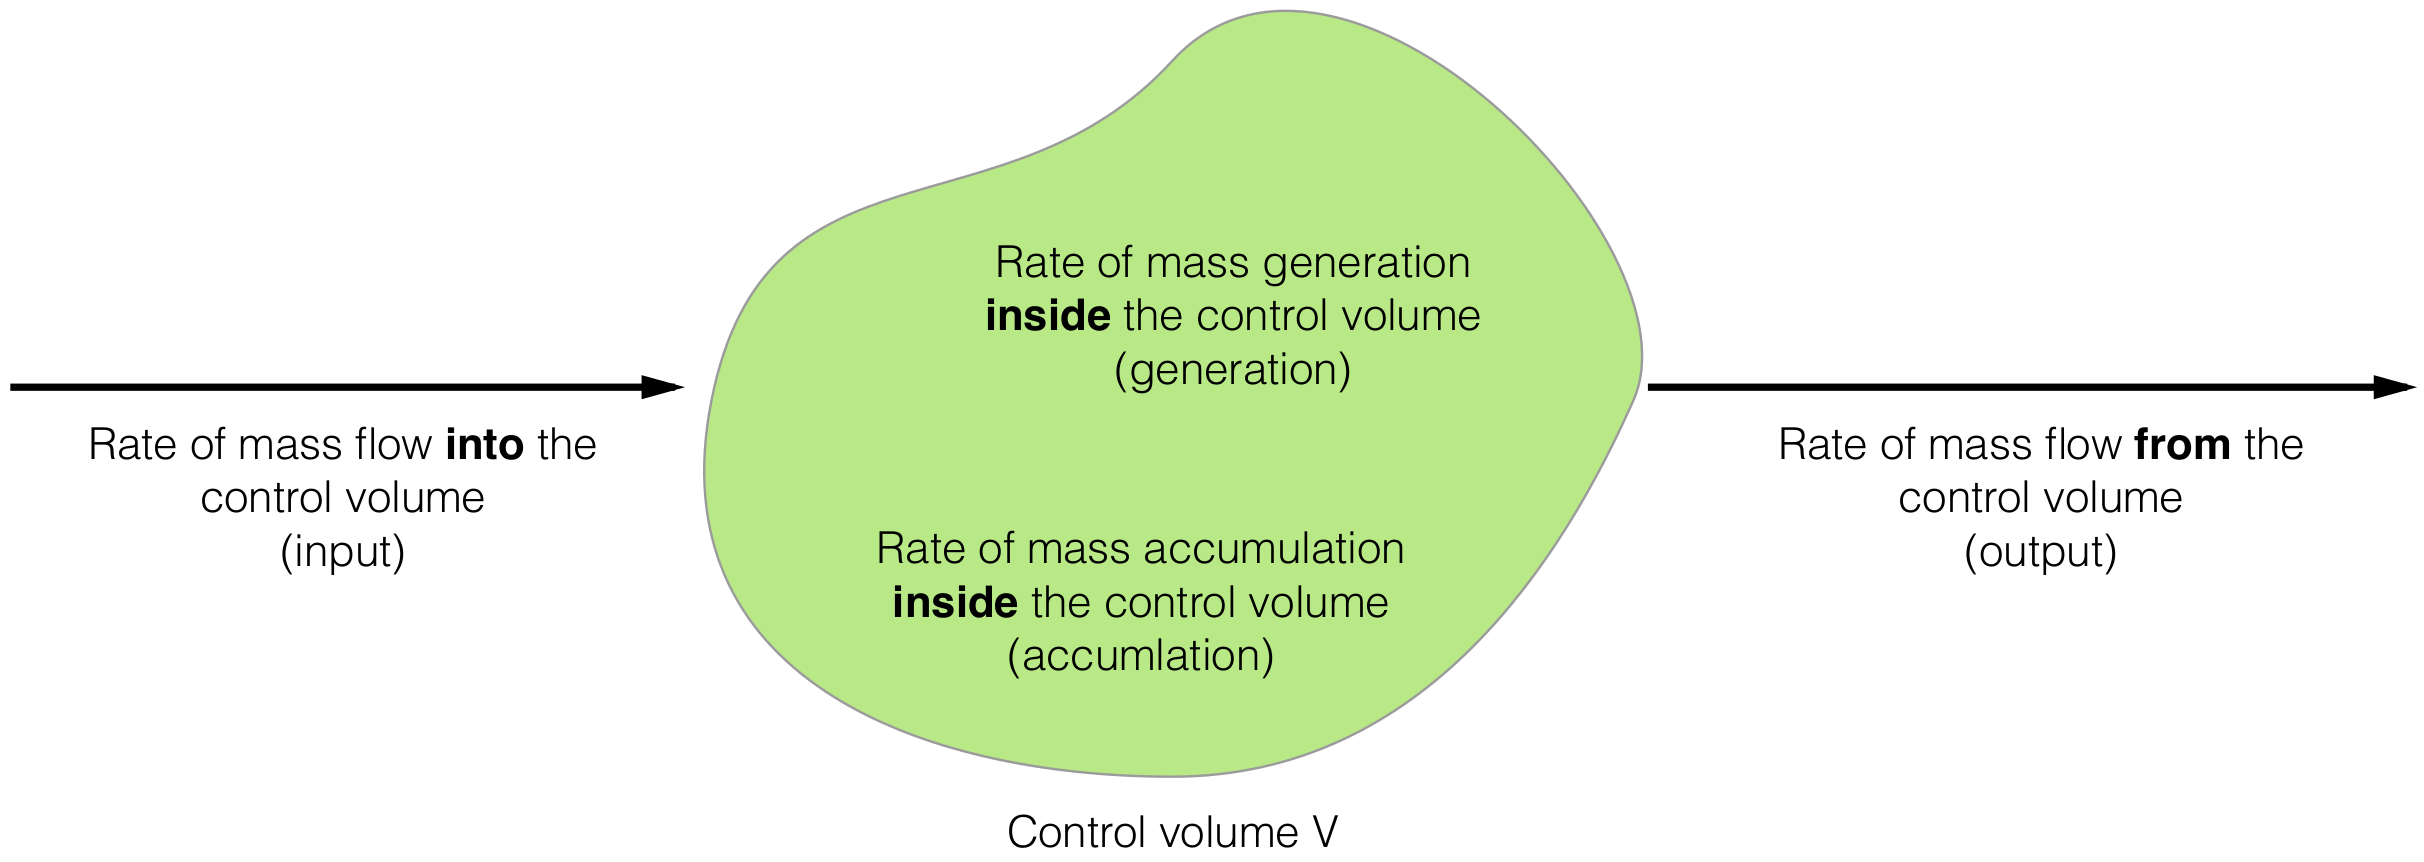
\includegraphics[width=1.00\textwidth]{Figure1.png}
%\end{center}
\caption{Schematic of an idealized control volume V. Total macroscopic material balance equations consist of four types of terms. Material flow into and from the control volume, material generation inside the control volume and material accumulation inside the control volume. The abundance of material can be measured using both a mass or mole basis.}
\label{fig:Carbon}
\end{figure}

%\FloatBarrier

Given an idealized control volume, the concentration of any species (metabolite) within will change according to four processes: flow in, flow out, generation, and consumption.
We can define a mass flow rate $\dot{m}_s$ for each stream into or out of the control volume, and a direction parameter $v_s$ such that $v_s=1$ for streams entering the control volume and $v_s=-1$ for streams exiting the control volume.
Furthermore, we can define generation minus consumption as net generation $\dot{m}_{gen}$, and the overall resulting change in concentration as accumulation $\dot{m}_{acc}$.
This gives us:

\begin{equation}
    \dot{m}_{acc}=\sum_{s=1}^{\mathcal{S}}v_s \dot{m}_s+\dot{m}_{gen}
\end{equation}
However, we can also write a mole balance in the same way:

\begin{equation}
    \dot{n}_{acc}=\sum_{s=1}^{\mathcal{S}}v_s \dot{n}_s+\dot{n}_{gen}
\end{equation}
Conservation of mass dictates that net mass generation is zero $\dot{m}_{gen}=0$, but no such law exists for a mole balance $\dot{n}_{gen}\neq 0$.
We can write a mole balance around an individual species as well:

\begin{equation}
    \dot{n}_{j,acc}=\sum_{s=1}^{\mathcal{S}}v_s \dot{n}_s x_{j,s}+\dot{n}_{j,gen}\qquad{j=1,2,\hdots,\mathcal{M}}
\end{equation}
where $x_{j,s}$ is the mole fraction of species $j$ in stream $s$.
We can also construct a balance using volumetric flow rate $F_s$ as a basis for each stream, in which case mole fraction will be replaced by species concentration $C_{j,s}$:

\begin{equation}
    \frac{d}{dt}\left(C_j V\right)=\sum_{s=1}^{\mathcal{S}}v_s F_s C_{j,s}+\dot{n}_{j,gen}\qquad{j=1,2,\hdots,\mathcal{M}}
\end{equation}
Here the mole rate of accumulation of species $j$ is equal to the rate of change of the species concentration times the volume.

To better understand how moles of a species can be generated in a cell, we must consider the stoichiometry of cellular metabolism. Generally, cells consume substrates $S_1,S_2,\hdots,S_N$ to produce products $P_1,P_2,\hdots,P_M$, as well as more cells $X$:

\begin{equation}
    \sum_{i=1}^{N}Y_{XS_i}S_i\overset{\mu}{\longrightarrow}X+\sum_{j=1}^{M}Y_{XP_j}P_j
\end{equation}
$Y_{Xj}$ are yield coefficients, which relate the consumption or production of a species to $\mu$, the specific growth rate of cells.
If a species is a substrate, $Y_{Xj}$ represents how much of that substrate is consumed in the production of one unit of cells.
$Y_{Xj}<0$ for all substrates, and $Y_{Xj}>0$ for all products.
Thus, $Y_{XS_i}<0$ and $Y_{XP_j}>0$ in the equation above.
This is the overall stoichiometry from substrates to products, a lumped version of all the chemical reactions that occur in the cell.


\begin{equation}
    \dot{n}_{j,gen}=\left(\sum_{r=1}^\mathcal{R}\sigma_{j,r}\hat{r}_r\right)V+\left(\sum_{k=1}^\mathcal{T}\tau_{j,k}q_k\right)XV
\end{equation}

\begin{equation}
    \frac{d}{dt}\left(C_j V\right)=\sum_{s=1}^{\mathcal{S}}v_s F_s C_{j,s}+\left(\sum_{r=1}^\mathcal{R}\sigma_{j,r}\hat{r}_r\right)V+\left(\sum_{k=1}^\mathcal{T}\tau_{j,k}q_k\right)XV\qquad{j=1,2,\hdots,\mathcal{M}}
\end{equation}




\clearpage

\section*{Extracellular balances}

\begin{flalign}
	\frac{dC_j}{dt}&=\sum_{s=1}^{\mathcal{S}}v_s D_s C_{j,s}+\left(\sum_{r=1}^{\mathcal{R}}\sigma_{j,r}\hat{r}_r\right)+\left(\sum_{k=1}^{\mathcal{T}}\tau_{j,k}q_k\right)X-\frac{C_j}{V}\frac{dV}{dt}\phantom{abc}j=1,2,\ldots,\mathcal{M}\\[10pt]
	\frac{dX}{dt}&=\sum_{s=1}^{\mathcal{S}}v_s D_s X_s+\left(\mu-k_d\right)X-\frac{X}{V}\frac{dV}{dt}\\[10pt]
	\frac{dV}{dt}&=\sum_{s=1}^{\mathcal{S}}v_s\frac{\rho_s}{\rho}F_s-\frac{V}{\rho}\frac{d\rho}{dt}\\[10pt]
	D_s&\equiv\frac{F_s}{V}
\end{flalign}

\clearpage

\section*{Batch cultures}

A batch process is defined by the absence of flow in or out of the reactor:

\begin{equation}\label{eqn:batch-definition}
    F_{in}=F_{out}=0\phantom{abc}\therefore\phantom{abc}D_{in}=D_{out}=0
\end{equation}

This results in a simplification of our extracellular balances:

\begin{flalign}
	\frac{dS}{dt}&=-\left(\frac{\mu}{Y_{XS}}+m_S\right)X\\[10pt]
	\frac{dX}{dt}&=\left(\mu-k_d\right)X\\[10pt]
	\frac{dV}{dt}&=0
\end{flalign}

\clearpage

\section*{Solving the system of ODEs}

We used ordinary differential equations (ODEs) to model the time evolution of metabolite ($x_{i}$) and scaled enzyme abundance ($\epsilon_{i}$) in hypothetical cell-free metabolic networks:
\begin{eqnarray}
	\frac{dx_{i}}{dt} & = & \sum_{j=1}^{\mathcal{R}}\sigma_{ij}r_{j}\left(\mathbf{x},\mathbf{\epsilon},\mathbf{k}\right)\qquad{i=1,2,\hdots,\mathcal{M}}\\
	\frac{d\epsilon_{i}}{dt} & = & -\lambda_{i}\epsilon_{i}\qquad{i=1,2,\hdots,\mathcal{E}}
\end{eqnarray}where $\mathcal{R}$ denotes the number of reactions, $\mathcal{M}$ denotes the number of metabolites and $\mathcal{E}$ denotes the number of enzymes in the model.
The quantity $r_{j}\left(\mathbf{x},\mathbf{\epsilon},\mathbf{k}\right)$ denotes the rate of reaction $j$.
Typically, reaction $j$ is a non-linear function of metabolite and enzyme abundance, as well as unknown kinetic parameters $\mathbf{k}$ ($\mathcal{K}\times{1}$).
The quantity $\sigma_{ij}$ denotes the stoichiometric coefficient for species $i$ in reaction $j$.
If $\sigma_{ij}>0$, metabolite $i$ is produced by reaction $j$.
Conversely, if $\sigma_{ij}<0$, metabolite $i$ is consumed by reaction $j$, while $\sigma_{ij}=0$ indicates metabolite $i$ is not connected with reaction $j$.
Lastly, $\lambda_{i}$ denotes the scaled enzyme activity decay constant.
The system material balances were subject to the initial conditions $\mathbf{x}\left(t_{o}\right)=\mathbf{x}_{o}$ and $\mathbf{\epsilon}\left(t_{o}\right)=\mathbf{1}$ (initially we have 100\% cell-free enzyme abundance).

\clearpage

\section*{Heuristic optimization}

After solving the equations, we can calculate a variety of metrics to evaluate the model solution.
One of these is the cost function, equal to the sum-squared-error between experimental data and model predictions:
\begin{equation}\label{eqn:cost-function}
    \texttt{cost}=\sum_{i=1}^{\mathcal{D}}\left[\frac{w_i}{\mathcal{Y}_{i}^2}\sum_{j=1}^{\mathcal{T}_i}\bigg(y_{ij}-x_{i}|_{t(j)}\bigg)^2 \right]
\end{equation}
Here, $x_{i}$ are the simulated species values (the solution to the model ODEs), and $y_{ij}$ are the experimmental data against which we will compare these simulations.
$i$ is an index for the number of species for which data exist (usually less than the total number of species).
$j$ refers to the time index for the experimental data, not the simulations.
Thus, in order to actually subtract our simulations from the data, we must interpolate them to fit the experimental time index: $x_{i}|_{t(j)}$.
The number of experimental timepoints ($\mathcal{T}_i$) can depend on which species is being considered, hence the subscript $i$.
We then calculate a sum-squared-error for each species, and sum across all species in the dataset ($i =$ 1 to $\mathcal{D}$).
However, each species' sum-squared-error is first normalized by the square of the maximal experimental value $\mathcal{Y}_{i}=\max_{j}\left(y_{ij}\right)$.
In addition, we can weight the various species' contributions to the overall cost: $w_i$ are arbitrary, and should be used to prioritize fitting certain species over others.

The model solution, and thus the value of the cost function, depend on the model parameters (rate maxima, saturation constants, and control parameters).

\clearpage

\section*{Materials and Methods}

\subsection*{Estimation of kinetic model parameters.}
We estimated an ensemble of diverse parameter sets using a constrained Markov Chain Monte Carlo (MCMC) random walk strategy.
Starting from a single best-fit parameter set estimated by inspection and literature,

We then perturbed each model parameter between an upper and lower bound that varied by parameter type:
\begin{equation}\label{eqn:parameter-perturbation}
    k_i^{new}=\min\left(\max\left(k_i \cdot \exp(a \cdot r_i),l_i\right),u_i\right)\qquad{i=1,2,\hdots,\mathcal{P}}
\end{equation}
where $\mathcal{P}$ denotes the number of parameters ($\mathcal{P}$~=~815), which includes 163 maximum reaction rates ($V^{max}$), 163 enzyme activity decay constants, 455 saturation constants ($K_{js}$), and 34 control parameters, $k_i^{new}$ denotes the new value of the $i^{th}$ parameter, $k_i$ denotes the current value of the $i^{th}$ parameter, $a$ denotes a distribution variance, $r_i$ denotes a random sample from the normal distribution, $l_i$ denotes the lower bound for that parameter type, and $u_i$ denotes the upper bound for that parameter type.

Model parameters were constrained by literature \textit{Milo:2009aa}.
The rate maximum for CAT transcription was calculated as 123 h$^{-1}$:
\begin{equation}\label{eqn:transcription_rate}
	k_{cat}^{TX}=\left(\frac{k_{TX}}{l_{mRNA}}\right)\cdot P
\end{equation}
where $k_{TX}$ denotes the average mRNA elongation rate (25 nt/s, \textit{Garamella:2016aa}), $l_{mRNA}$ denotes the CAT mRNA length (660 nt), and $P$ denotes the level of promoter activity (estimated at 0.9).

\subsection*{Calculation of carbon yield.}
The CAT carbon yield ($Y_{C}^{CAT}$) was calculated as the ratio of carbon produced as CAT divided by the carbon consumed as reactants:
\begin{equation}\label{eqn:yield-definition}
	Y_{C}^{CAT}=\frac{\Delta\texttt{CAT}\cdot C_{CAT}}{\displaystyle\sum_{i=1}^{\mathcal{R}}\Delta m_{i}\cdot C_i}
\end{equation}
where $\Delta\texttt{CAT}$ denotes the abundance of CAT produced, $C_{CAT}$ denotes carbon number of CAT, $\mathcal{R}$ denotes the number of reactants, $\Delta m_{i}$ denotes the amount of the $i^{th}$ reactant consumed, and $C_i$ denotes the carbon number of the $i^{th}$ reactant.

\subsection*{Calculation of energy efficiency.}
Energy efficiency was calculated as the ratio of CAT production to substrate consumption, both in terms of equivalent ATP molecules:
\begin{equation}\label{eqn:energy-efficiency-definition}
	{\rm Efficiency}=\frac{\Delta\texttt{CAT}\cdot \left(2\cdot\left(\rm {ATP}_{TX}+\rm {CTP}_{TX}+\rm {GTP}_{TX}+\rm {UTP}_{TX}\right)+\rm2\cdot\rm {ATP}_{TL}+\rm {GTP}_{TL}\right)}{\displaystyle\sum_{i=1}^{\mathcal{R}}\Delta m_{i}\cdot {\rm ATP}_i}
\end{equation}
where $\rm {ATP}_{TX}$, $\rm {CTP}_{TX}$, $\rm {GTP}_{TX}$, $\rm {UTP}_{TX}$ denote the stoichiometric coefficients of each energy species for CAT transcription, $\rm {ATP}_{TL}$, $\rm {GTP}_{TL}$ denote the stoichiometric coefficients of ATP and GTP for CAT translation, $\Delta m_{i}$ denotes the amount of the $i^{th}$ substrate consumed, and ${\rm ATP}_i$ denotes the equivalent ATP number of the $i^{th}$ substrate.
$\rm {ATP}_{TX}$ = 176, $\rm {CTP}_{TX}$ = 144, $\rm {GTP}_{TX}$ = 151, $\rm {UTP}_{TX}$ = 189, $\rm {ATP}_{TL}$ = 219, $\rm {GTP}_{TL}$ = 438, $\rm {ATP}_{GLC}$ = 21, $\rm {ATP}_{PYR}$ = 8, $\rm {ATP}_{LAC}$ = 9.5, $\rm {ATP}_{SUCC}$ = 11.5, $\rm {ATP}_{MAL}$ = 10.5.

\clearpage

%\begin{table}
%\centering
% \caption{Reference values for reaction rate maxima (V$_{max}$) from literature. V$_{max}$ values calculated from turnover numbers (K$_{cat}$) from literature, and a characteristic enzyme concentration of 167 nM. Characteristic rate maximum for all other reactions calculated as geometric mean of calculated rate maxima.}
% \renewcommand{\arraystretch}{1.3}
% \begin{tabular}{llrrr} \toprule
%\phantom{i}\textbf{Enzyme} & \textbf{Reaction} & \textbf{K$_{cat}$ (min$^{-1}$)} & 
% \textbf{V$_{max}$ (mM/h)} & \textbf{BNID \#} \\ \hline
%\phantom{i}Serine dehydrase & R\_ser\_deg & 10400 & 104 & 101119 \\ \hline
%\phantom{i}Isocitrate dehydrogenase & R\_icd & 11900 & 119 & 101152 \\ \hline
%\phantom{i}Lactate dehydrogenase & R\_ldh & 5800 & 58 & 101036 \\ \hline
%\smallskip
%\rule{0pt}{4.5ex}
%Aspartate transaminase & \parbox{1 cm}{R\_aspC, R\_tyr, R\_phe} & 25800 & 258 & 101108 \\ \hline
%\phantom{i}Enolase & R\_eno & 13200 & 132 & 101028 \\ \hline
%\smallskip
%\rule{0pt}{3ex}
%Pyruvate kinase & R\_pyk & 25000 & 250 & \parbox{1.4 cm}{101029 101030} \\ \hline
%\smallskip
%\rule{0pt}{3ex}
%Malic enzyme & \parbox{1 cm}{R\_maeA, R\_maeB} & 35400 & 354 & 101167 \\ \hline
%\phantom{i}Phosphofructokinase & R\_pfk & 554400 & 5544 & 104955 \\ \hline
%\phantom{i}Malate dehydrogenase & R\_mdh & 33000 & 330 & 101163 \\ \hline
%\phantom{i}Citrate Synthase & R\_gltA & 42000 & 420 & 101149 \\ \hline
%\smallskip
%\rule{0pt}{4.5ex}
%6PG dehydrogenase & \parbox{1 cm}{R\_zwf, R\_pgl, R\_gnd} &3200 & 32 & 101048 \\ \hline
%\phantom{i}Succinate dehydrogenase & R\_sdh & 121 & 1.21 & 101162 \\ \hline
%\phantom{i}Succinyl-coA synthetase & R\_sucCD & 4700 & 47 & 101158 \\ \hline
%\phantom{i}3PGA dehydrogenase & R\_gpm & 1100 & 11 & 101135 \\ \hline
%\phantom{i}PEP carboxylase & R\_ppc & 35400 & 354 & 101139 \\ \hline
%\phantom{i}3PGA kinase & R\_pgk & 4300 & 43 & 101016 \\ \hline
%\phantom{i}Characteristic rate maximum & & & 110 & \\ \bottomrule
% \end{tabular}
%\label{tbl:Rate_maxima}
%\end{table}

\clearpage

\end{document}
\grid
\grid
